\documentclass[a4paper,12pt]{article}
\usepackage{outline}
\usepackage{pmgraph}
\usepackage[normalem]{ulem}
\usepackage{comment} % enables the use of multi-line comments (\ifx \fi)
\usepackage{lipsum} %This package just generates Lorem Ipsum filler text.
\usepackage{fullpage} % changes the margin
\usepackage{listings}
\usepackage{color}
\usepackage{mdframed}
\usepackage{listings}
\usepackage{amssymb}
\usepackage{amsmath}
\usepackage{graphicx}
\graphicspath{ {../screenshots/} }
\renewcommand{\lstlistingname}{Code Block}% Listing -> Algorithm
\renewcommand{\lstlistlistingname}{List of \lstlistingname s}% List of Listings -> List of Algorithms

\linespread{1.5}
%--------------------Indention
\setlength{\parindent}{15pt}
\lstset{frame=shadowbox, rulesepcolor=\color{white}}
\mdfsetup{frametitlealignment=\center}
\lstset{
  numbers=left,
  stepnumber=1,
  firstnumber=1,
  numberfirstline=true
}

\begin{document}
\section*{Objective}

  \hspace{15pt}The purpose of this lab was to expand on the students familiarity of sequential circuits
  by exposing them to the inner workings of a binary counter. The lab manual guided the students
  through desgining a binary up-counter using Verilog. Once designing was complete, the design
  will be synthesized onto the FPGA board using a student edited UCF file. Finally, the lab
  will conclude with two important use cases for binary counters, namely clock frequency division
  and I/O debouncing.

\section*{Design}
% The order is
% clock_divider.v
% 4 seperate clock signals image
% half_adder.v
% up_counter.v
% up countere image
% clock divider was edited so Count was 26 bits wide
% top_level.v
% top_level.ucf
% swich_bounce.v
% noDebounce.v
% withDebounce.v

  \textbf{Experiment 1}
  
  \vspace{5pt}
  
  In \textbf{Experiment 1}, we described a synchronous sequential circuit and loaded it onto the FBGA board. We also, gained experienced with counters and clock frequency 
  division.
  
  In this first block of code, we designed a clock divider which would divide the clock into different cycles. This design was synthesized and implemented onto the FBGA board.

  \lstinputlisting[language=Verilog,,caption=Clock Divider ]{../code/clock_divider.v}
  
  \textbf{Experiment 2}

  Next, we designed a simple half adder that would take in two inputs and outputs a Sum and Cout.

  \lstinputlisting[language=Verilog,,caption=Half Adder ]{../code/half_adder.v}
  
  The next design was an up counter. The design implemented and utilized four half adders that were just created. The half adders were used to incrementally add the bits 
  together. The reset would reset the count back to zero. The counter would only increment if the enable was on high. 

  \lstinputlisting[language=Verilog,,caption=Up Counter ]{../code/up_counter.v}
  
  In the next two blocks of code, a Top Level Verilog design was created as well as an accompanying UCF file. The Verilog design first described a MUX that would select a clock signal based on the values of the switch. The clock signals were divided by our clock divider module. We also instantiated four separate up counter modules in order to count up four bits that would output to four separate LEDs.
  
  The UCF file took the Verilog file and synthesized in a way such that the FBGA board would understand. The outputs of the up counter were connected to the LEDs on the FBGA board. The switches were connected to two of the switches on the board. The reset was connected to the South button and enable was wired to North.  

  \lstinputlisting[language=Verilog,,caption=Top Level (Verilog) ]{../code/top_level.v}

  \lstinputlisting[language=Verilog,,caption=Top Level (UCF) ]{../code/top_level.ucf}

  \textbf{Experiment 3}
  
  For the switch bounce and no denounce tests, the code was given and tested.
  
  The following is the design given for with debounce. The input wire goes into two flip flops in order to synchronize the signal and eliminate electrical chatter. Then the 
  signal goes into a binary counter. The LEDs correctly incremented based on the number of times the button was pressed. 

  \lstinputlisting[language=Verilog,,caption=With Debounce ]{../code/withDebounce.v}

\section*{Results}

  \textbf{Experiment 1}
  
  This is the results for the clock divider design displayed on the Logic Analyzer provided in lab. It displays the different frequencys of the output COUNT, and the results of clock division.

  % Figure with caption
  \newpage
   \begin{figure}[h]
    \begin{center}
      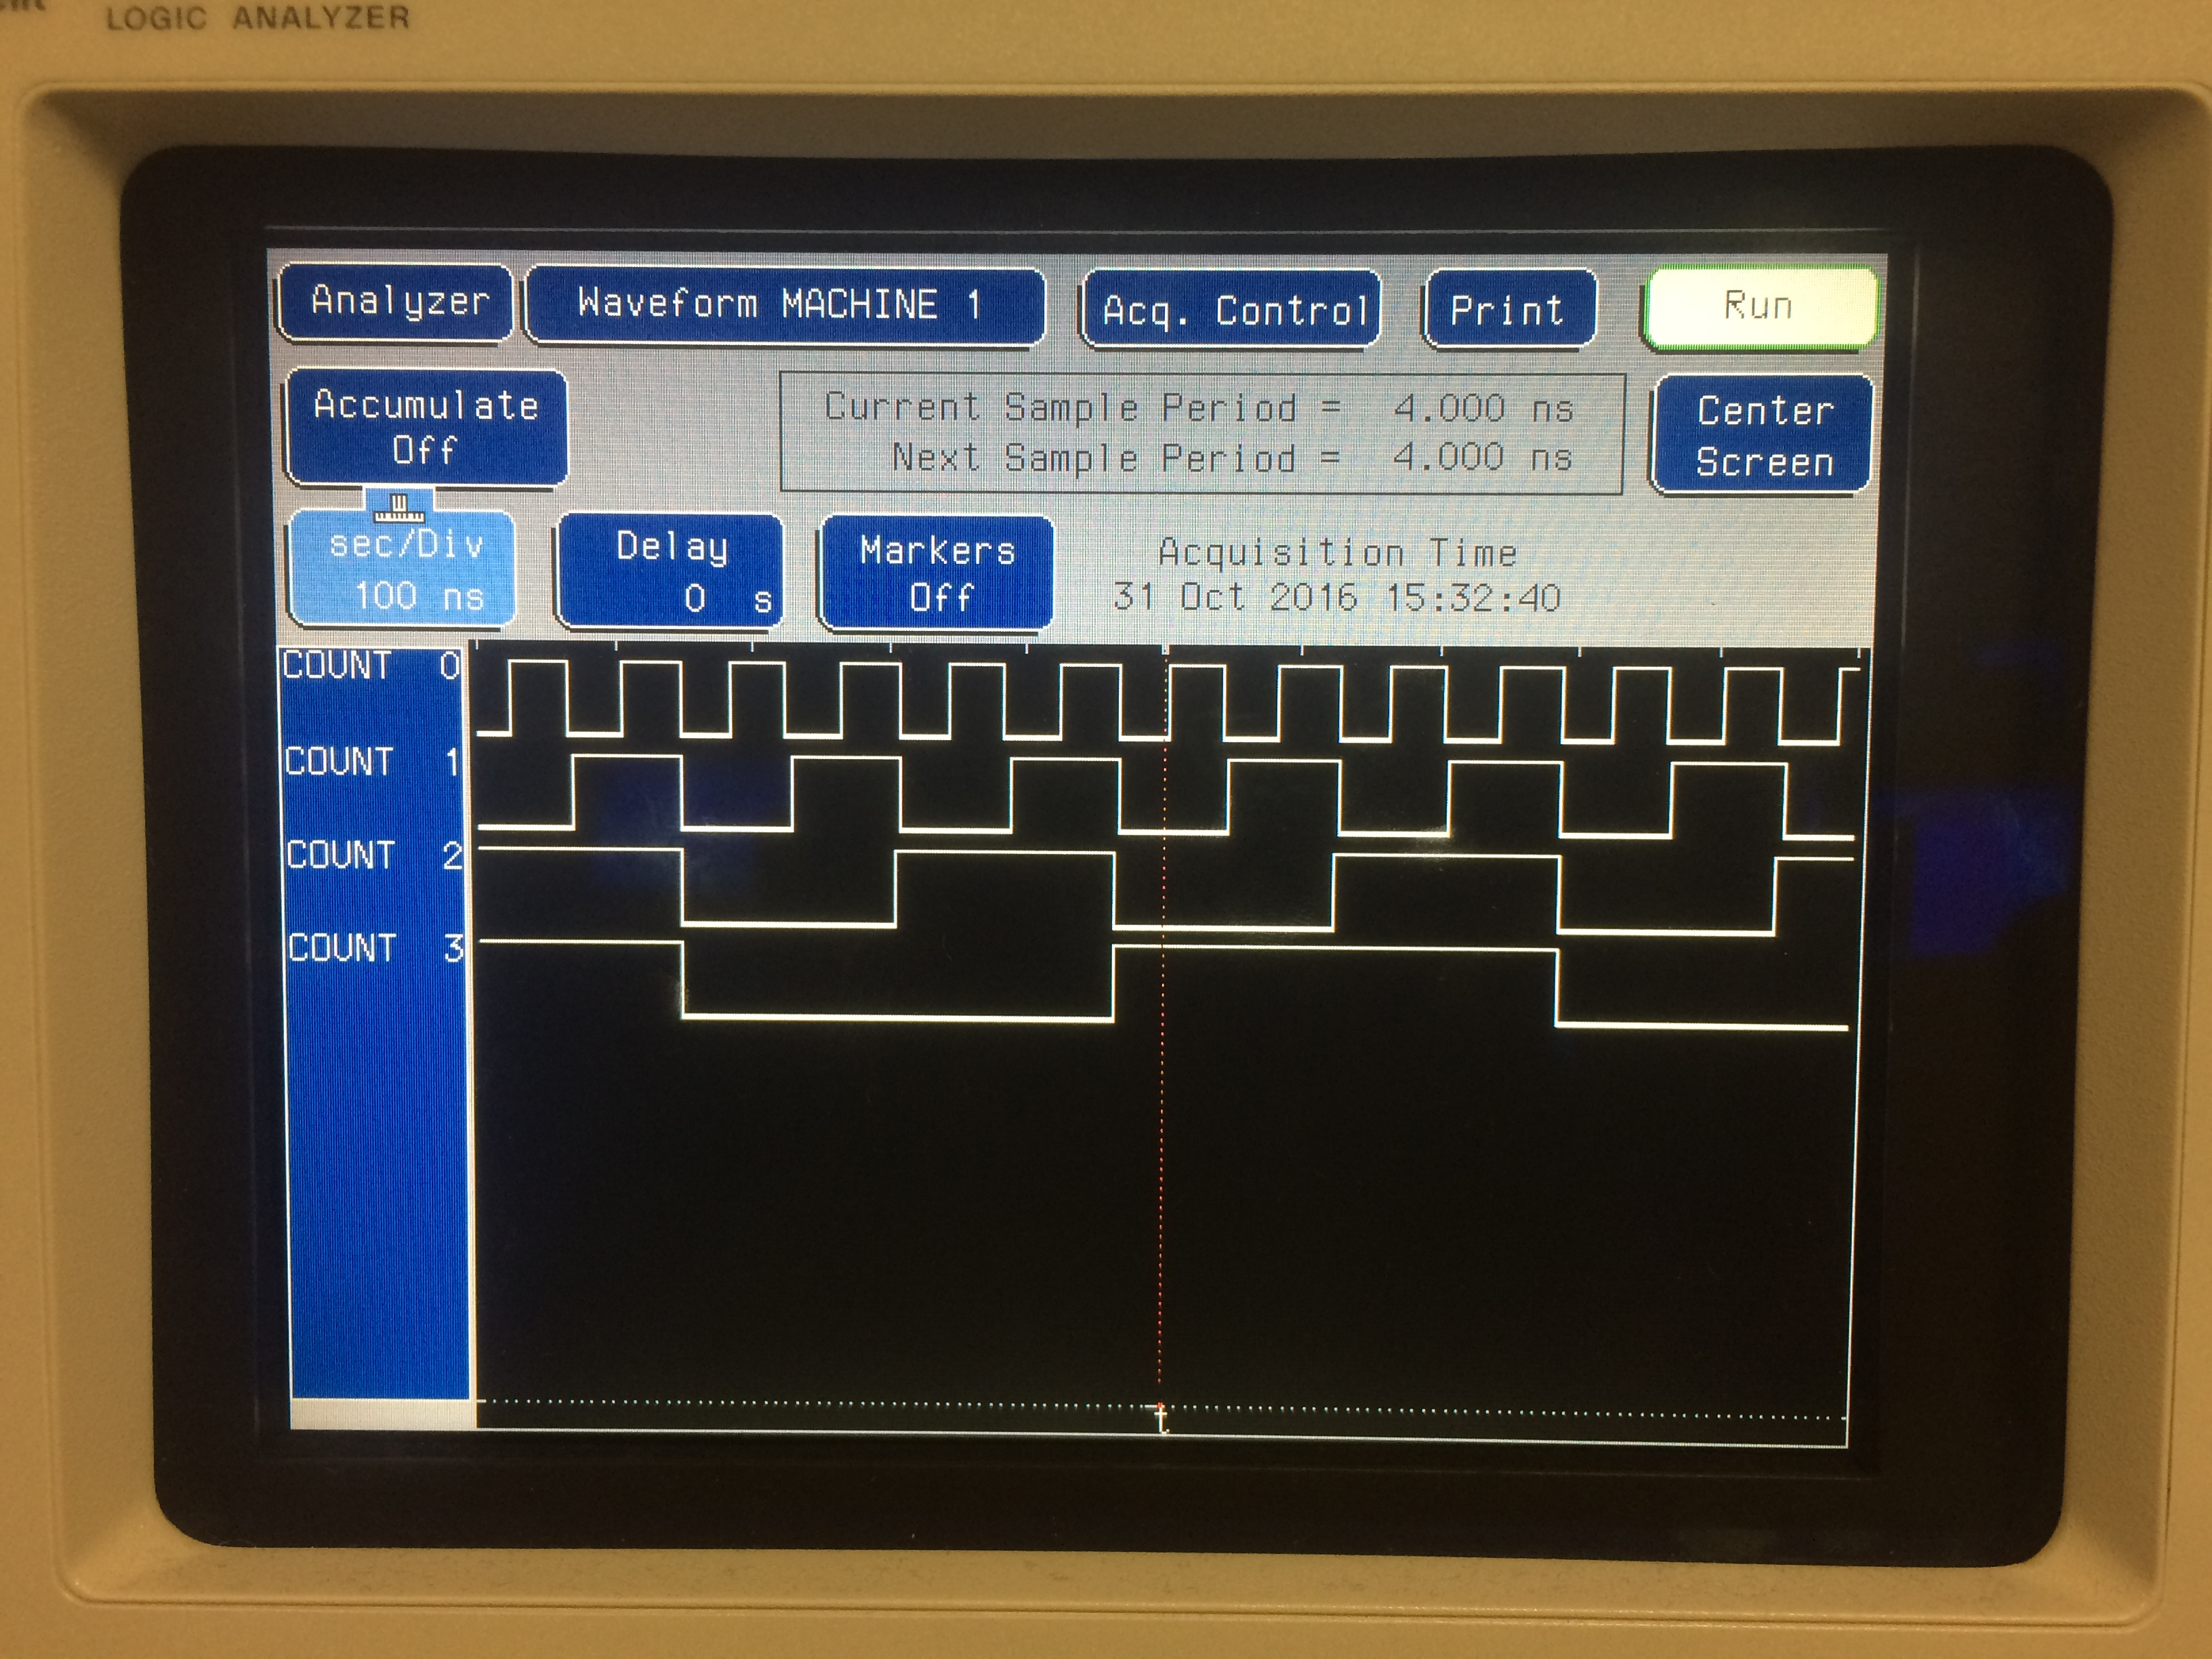
\includegraphics[scale=.08]{IMG_8620.JPG}
      \caption{\textit{Clock Divider on Logic Analyzer}}
    \end{center}
  \end{figure}
  
  In the next figure, the period for each clock cycle was calculated by determining the difference between the green and yellow. In this case, COUNT3 clock cycle was calculated. 
  
  \begin{figure}[h]
    \begin{center}
      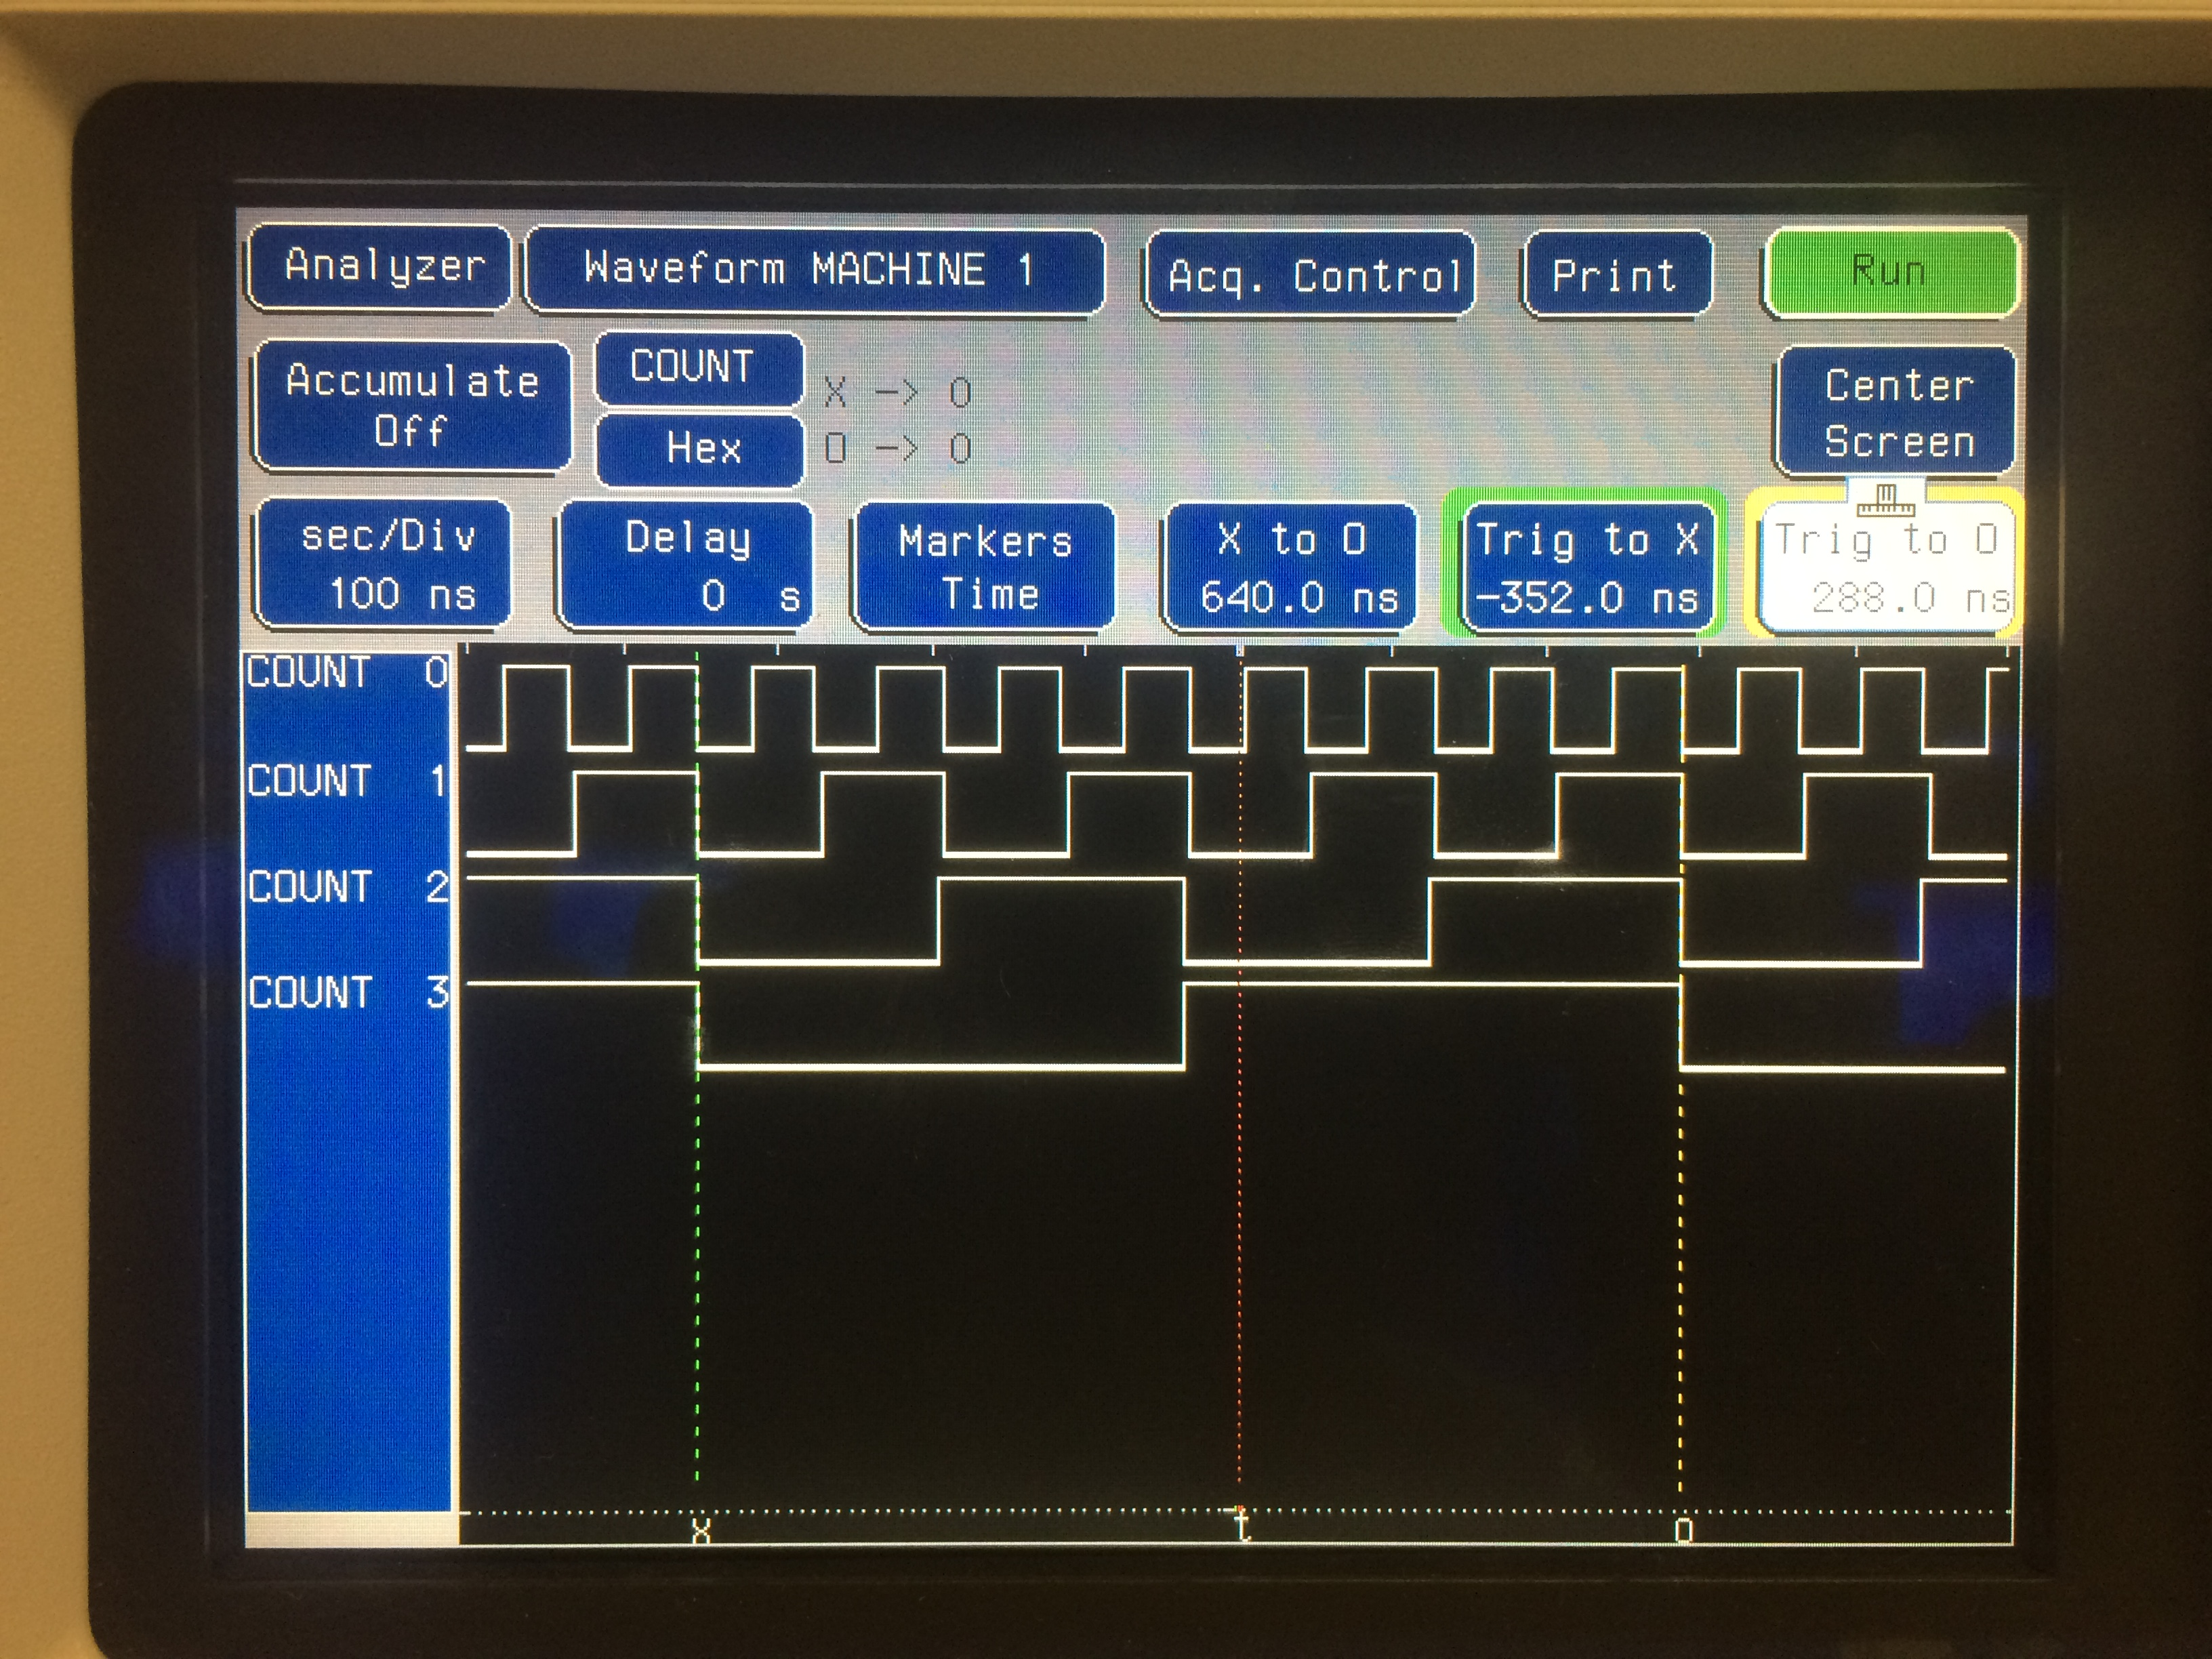
\includegraphics[scale=.08]{IMG_8621.JPG}
      \caption{\textit{Clock Divider with Distance Analysis}}
    \end{center}
  \end{figure}
  \newpage
  
  This figure, we modified the settings on the Logic Analyzer in order to display the hexadecimal values of the COUNT ALL.
  
  \begin{figure}[h]
    \begin{center}
      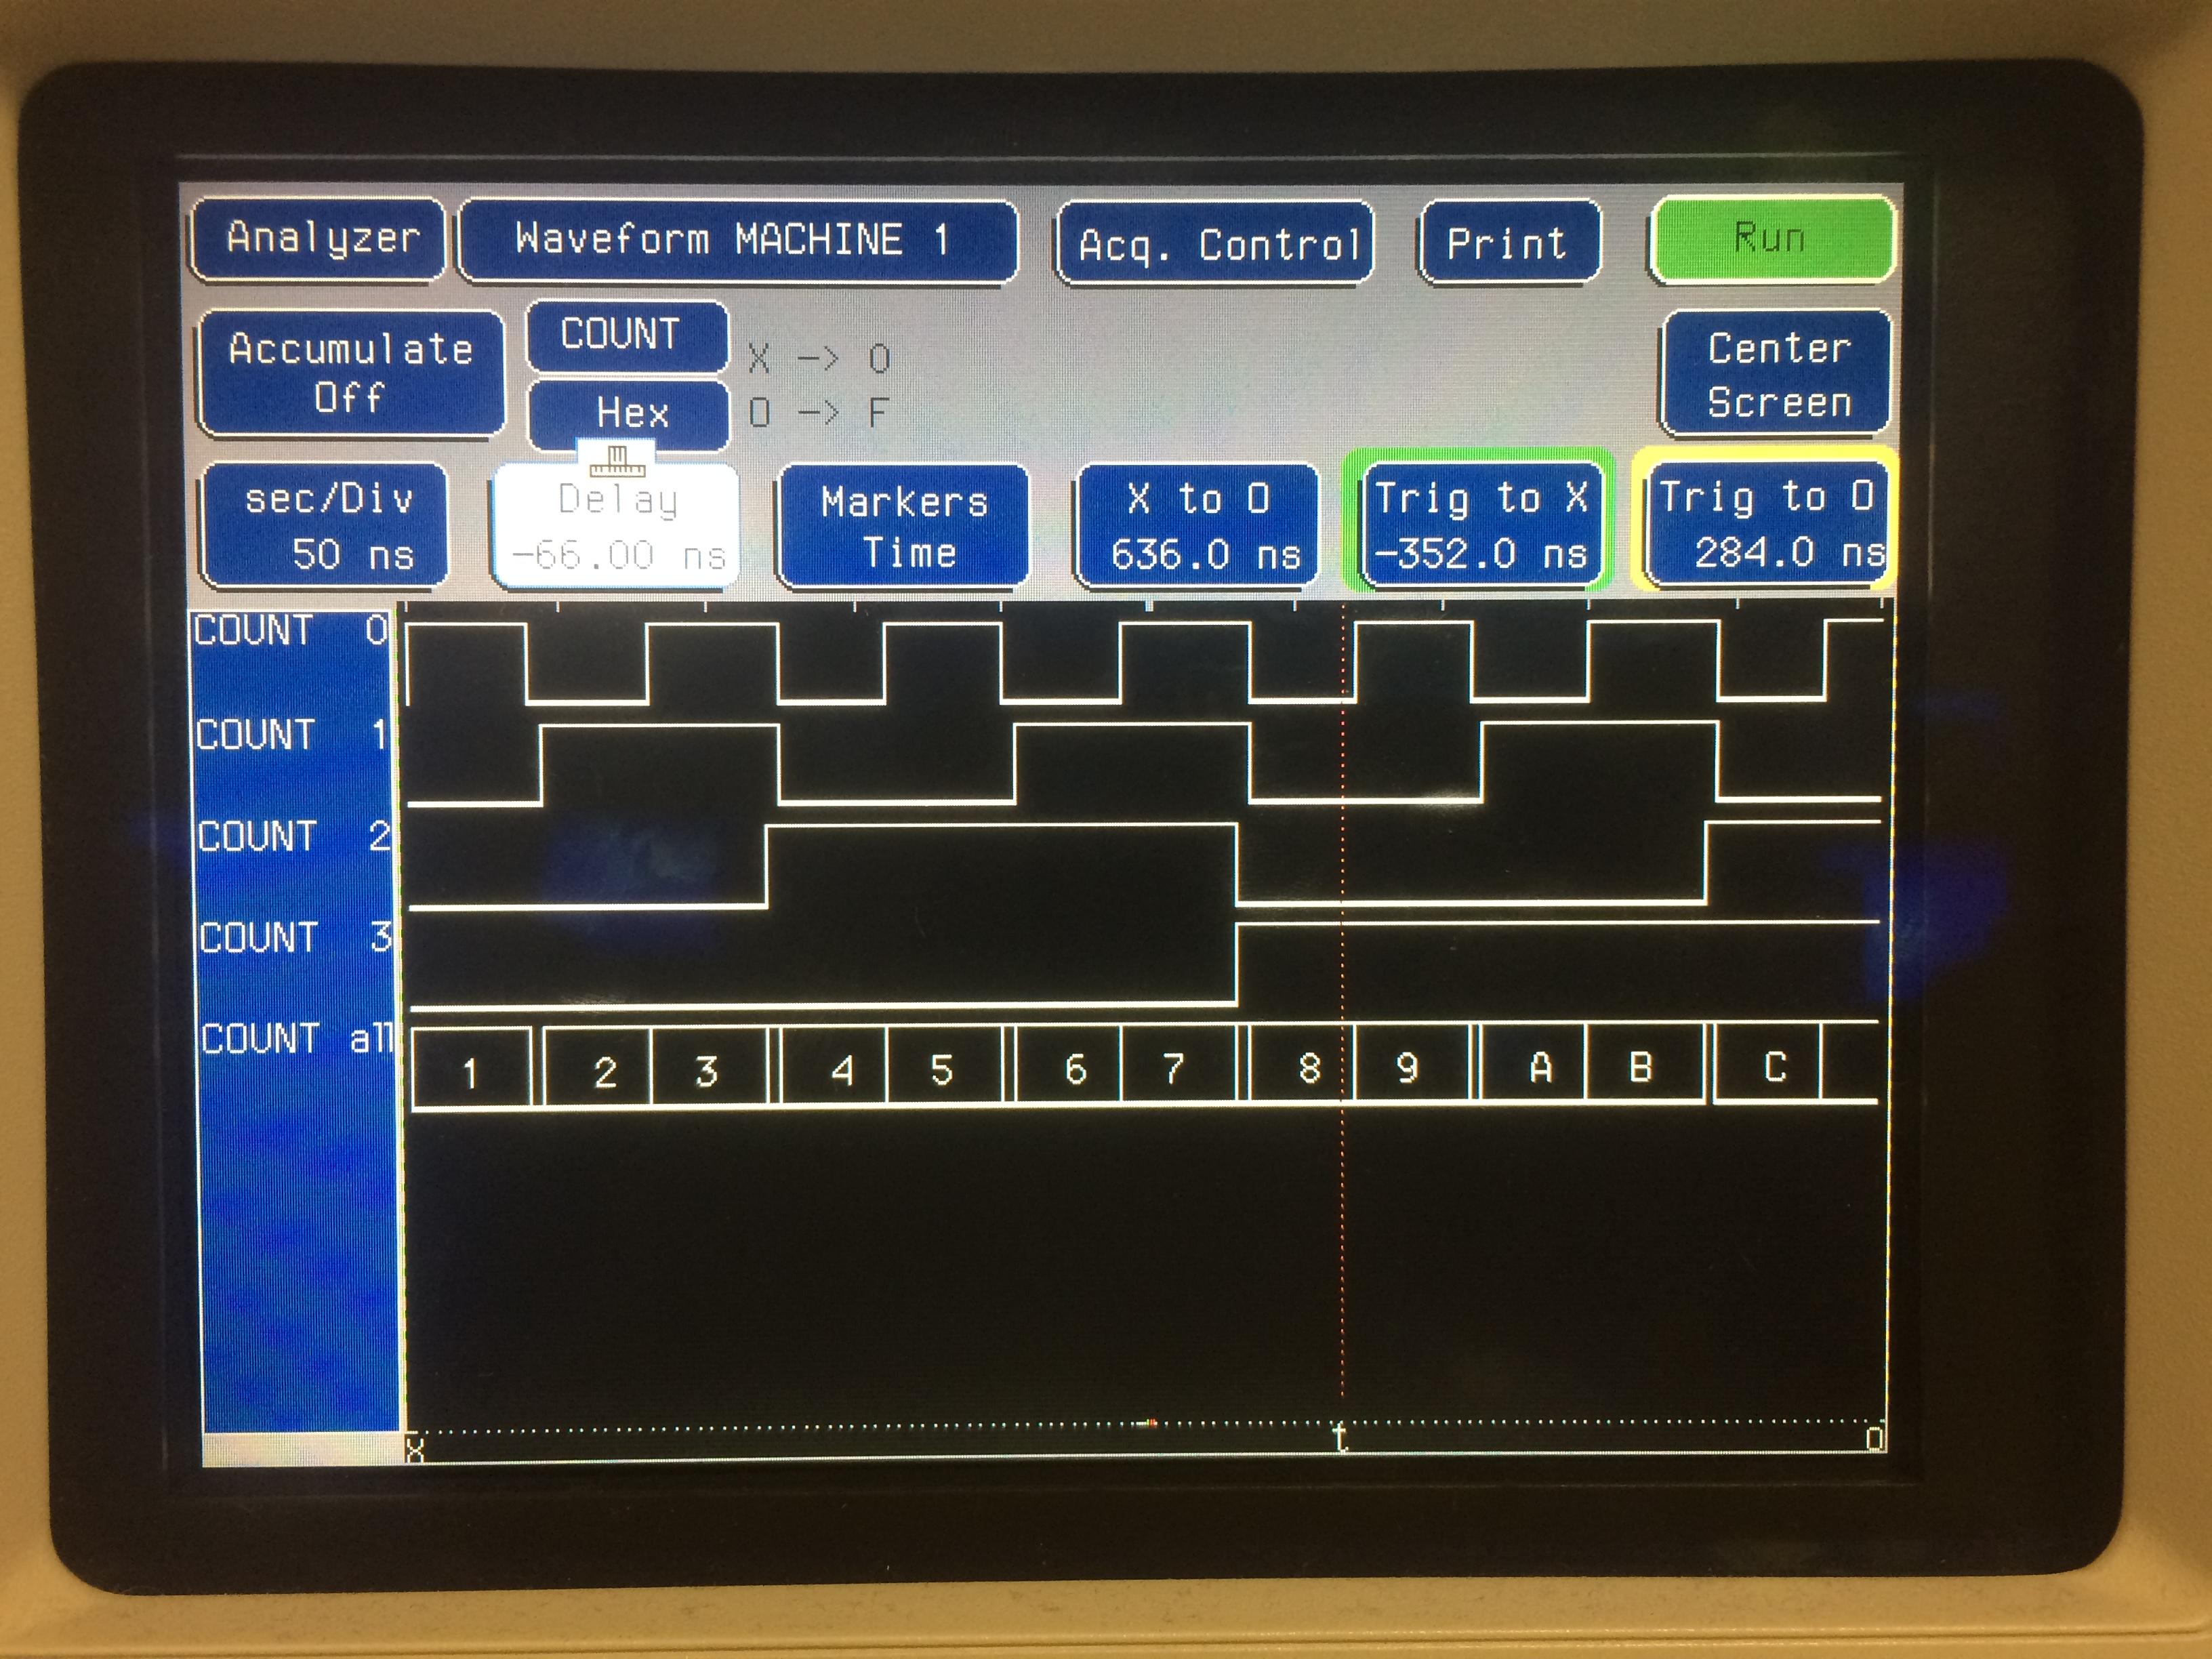
\includegraphics[scale=.08]{IMG_8622.JPG}
      \caption{\textit{Clock Divider with Count All Shown with Delay}}
    \end{center}
  \end{figure}
  
  The following is the result of the up counter being displayed in hexadecimal form.
  
  \begin{figure}[h]
    \begin{center}
      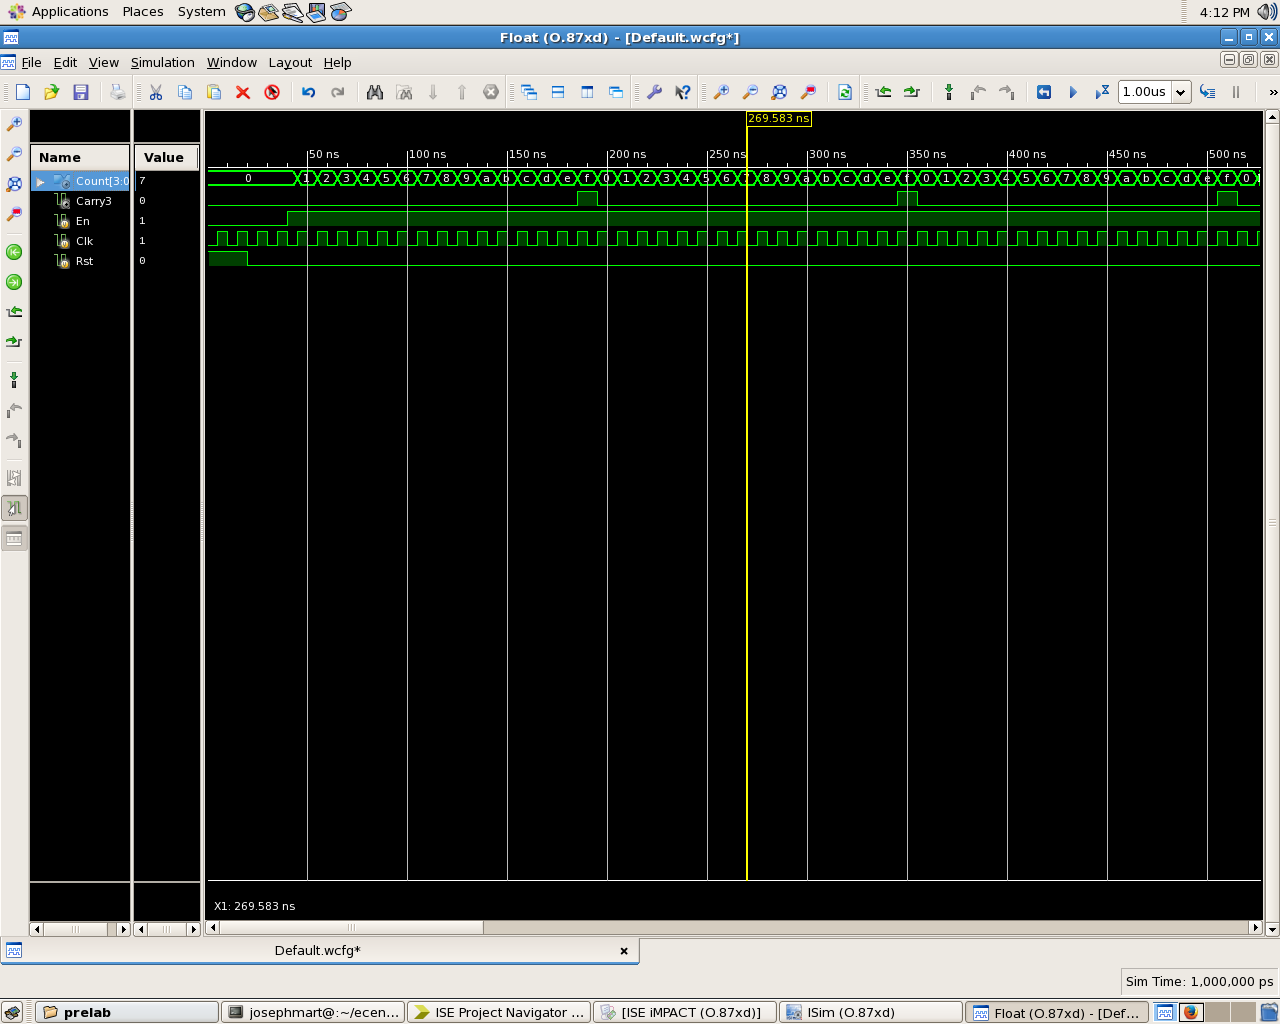
\includegraphics[scale=.18]{2_2_e.png}
      \caption{\textit{Up Counter}}
    \end{center}
  \end{figure}

  \newpage
  
  The following was the zoomed in version of the previous image in order to determine the period for the maximum value of the up counter (195 ns)
  
  \begin{figure}[h]
    \begin{center}
      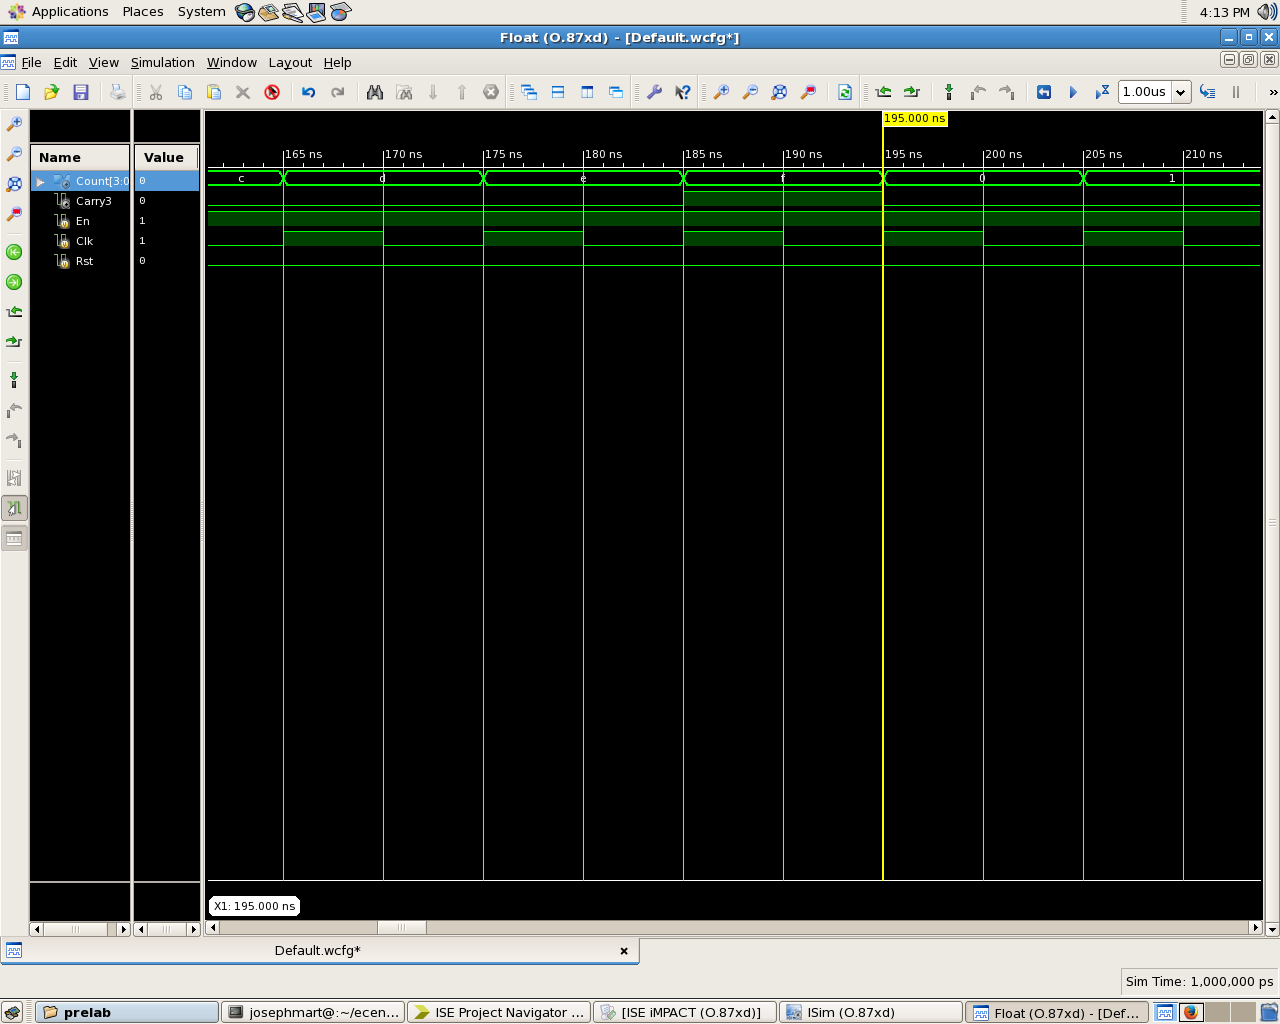
\includegraphics[scale=.18]{RollOver.png}
      \caption{\textit{Roll Over}}
    \end{center}
  \end{figure}
  
  In this image, the Count bit width was changed from 5 bits to 26 bits.
  
  \begin{figure}[h]
    \begin{center}
      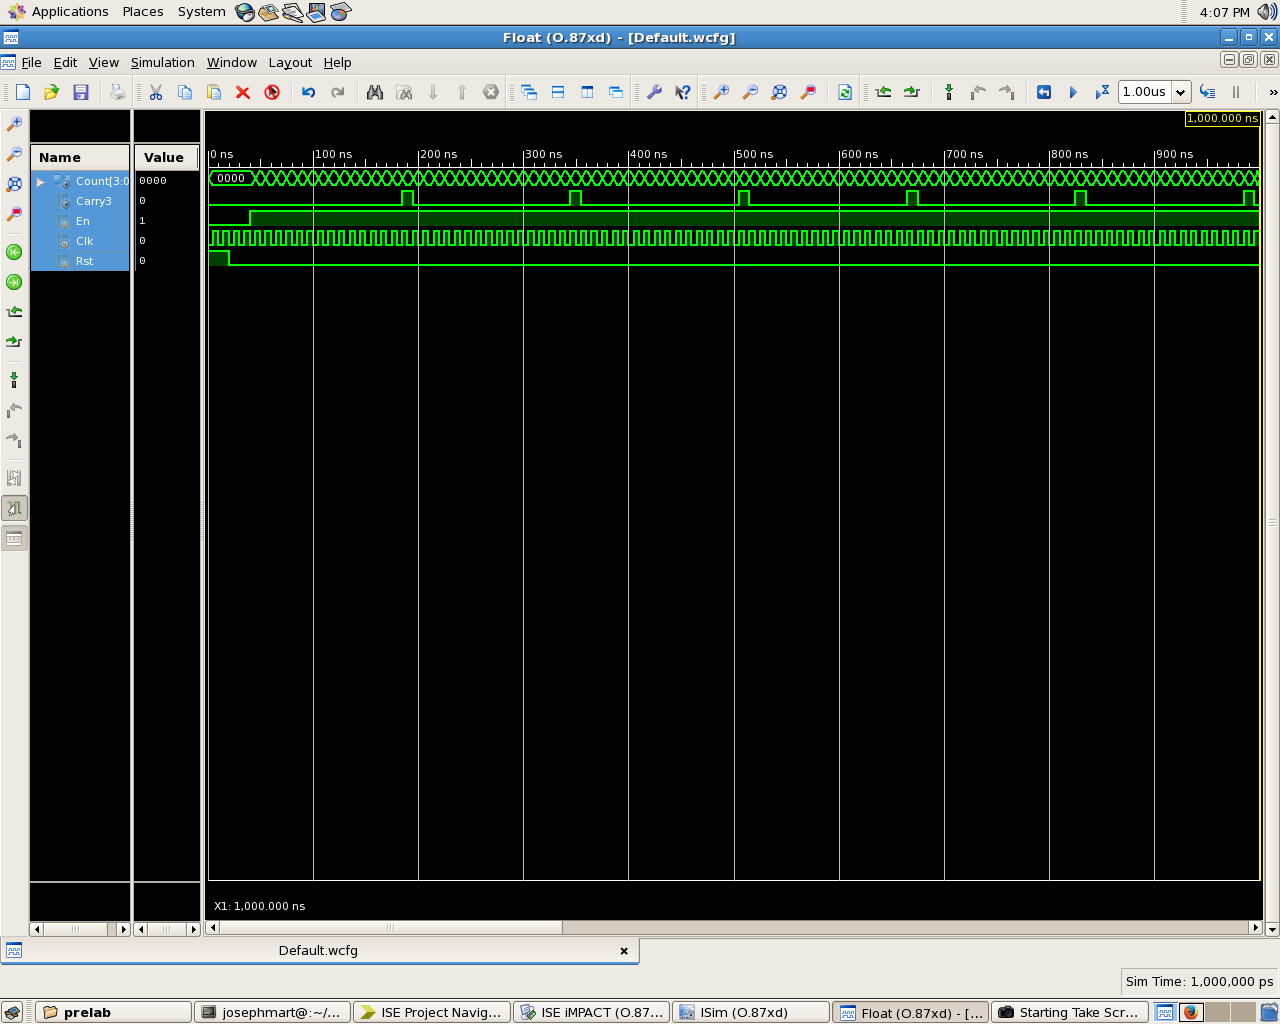
\includegraphics[scale=.18]{up_Count_waveform.png}
      \caption{\textit{Up Counter with 26 Bits}}
    \end{center}
  \end{figure}
  \newpage
  
  Electrical chatter of the Switch Bounce is visible in this final figure.
  
  \begin{figure}[h]
    \begin{center}
      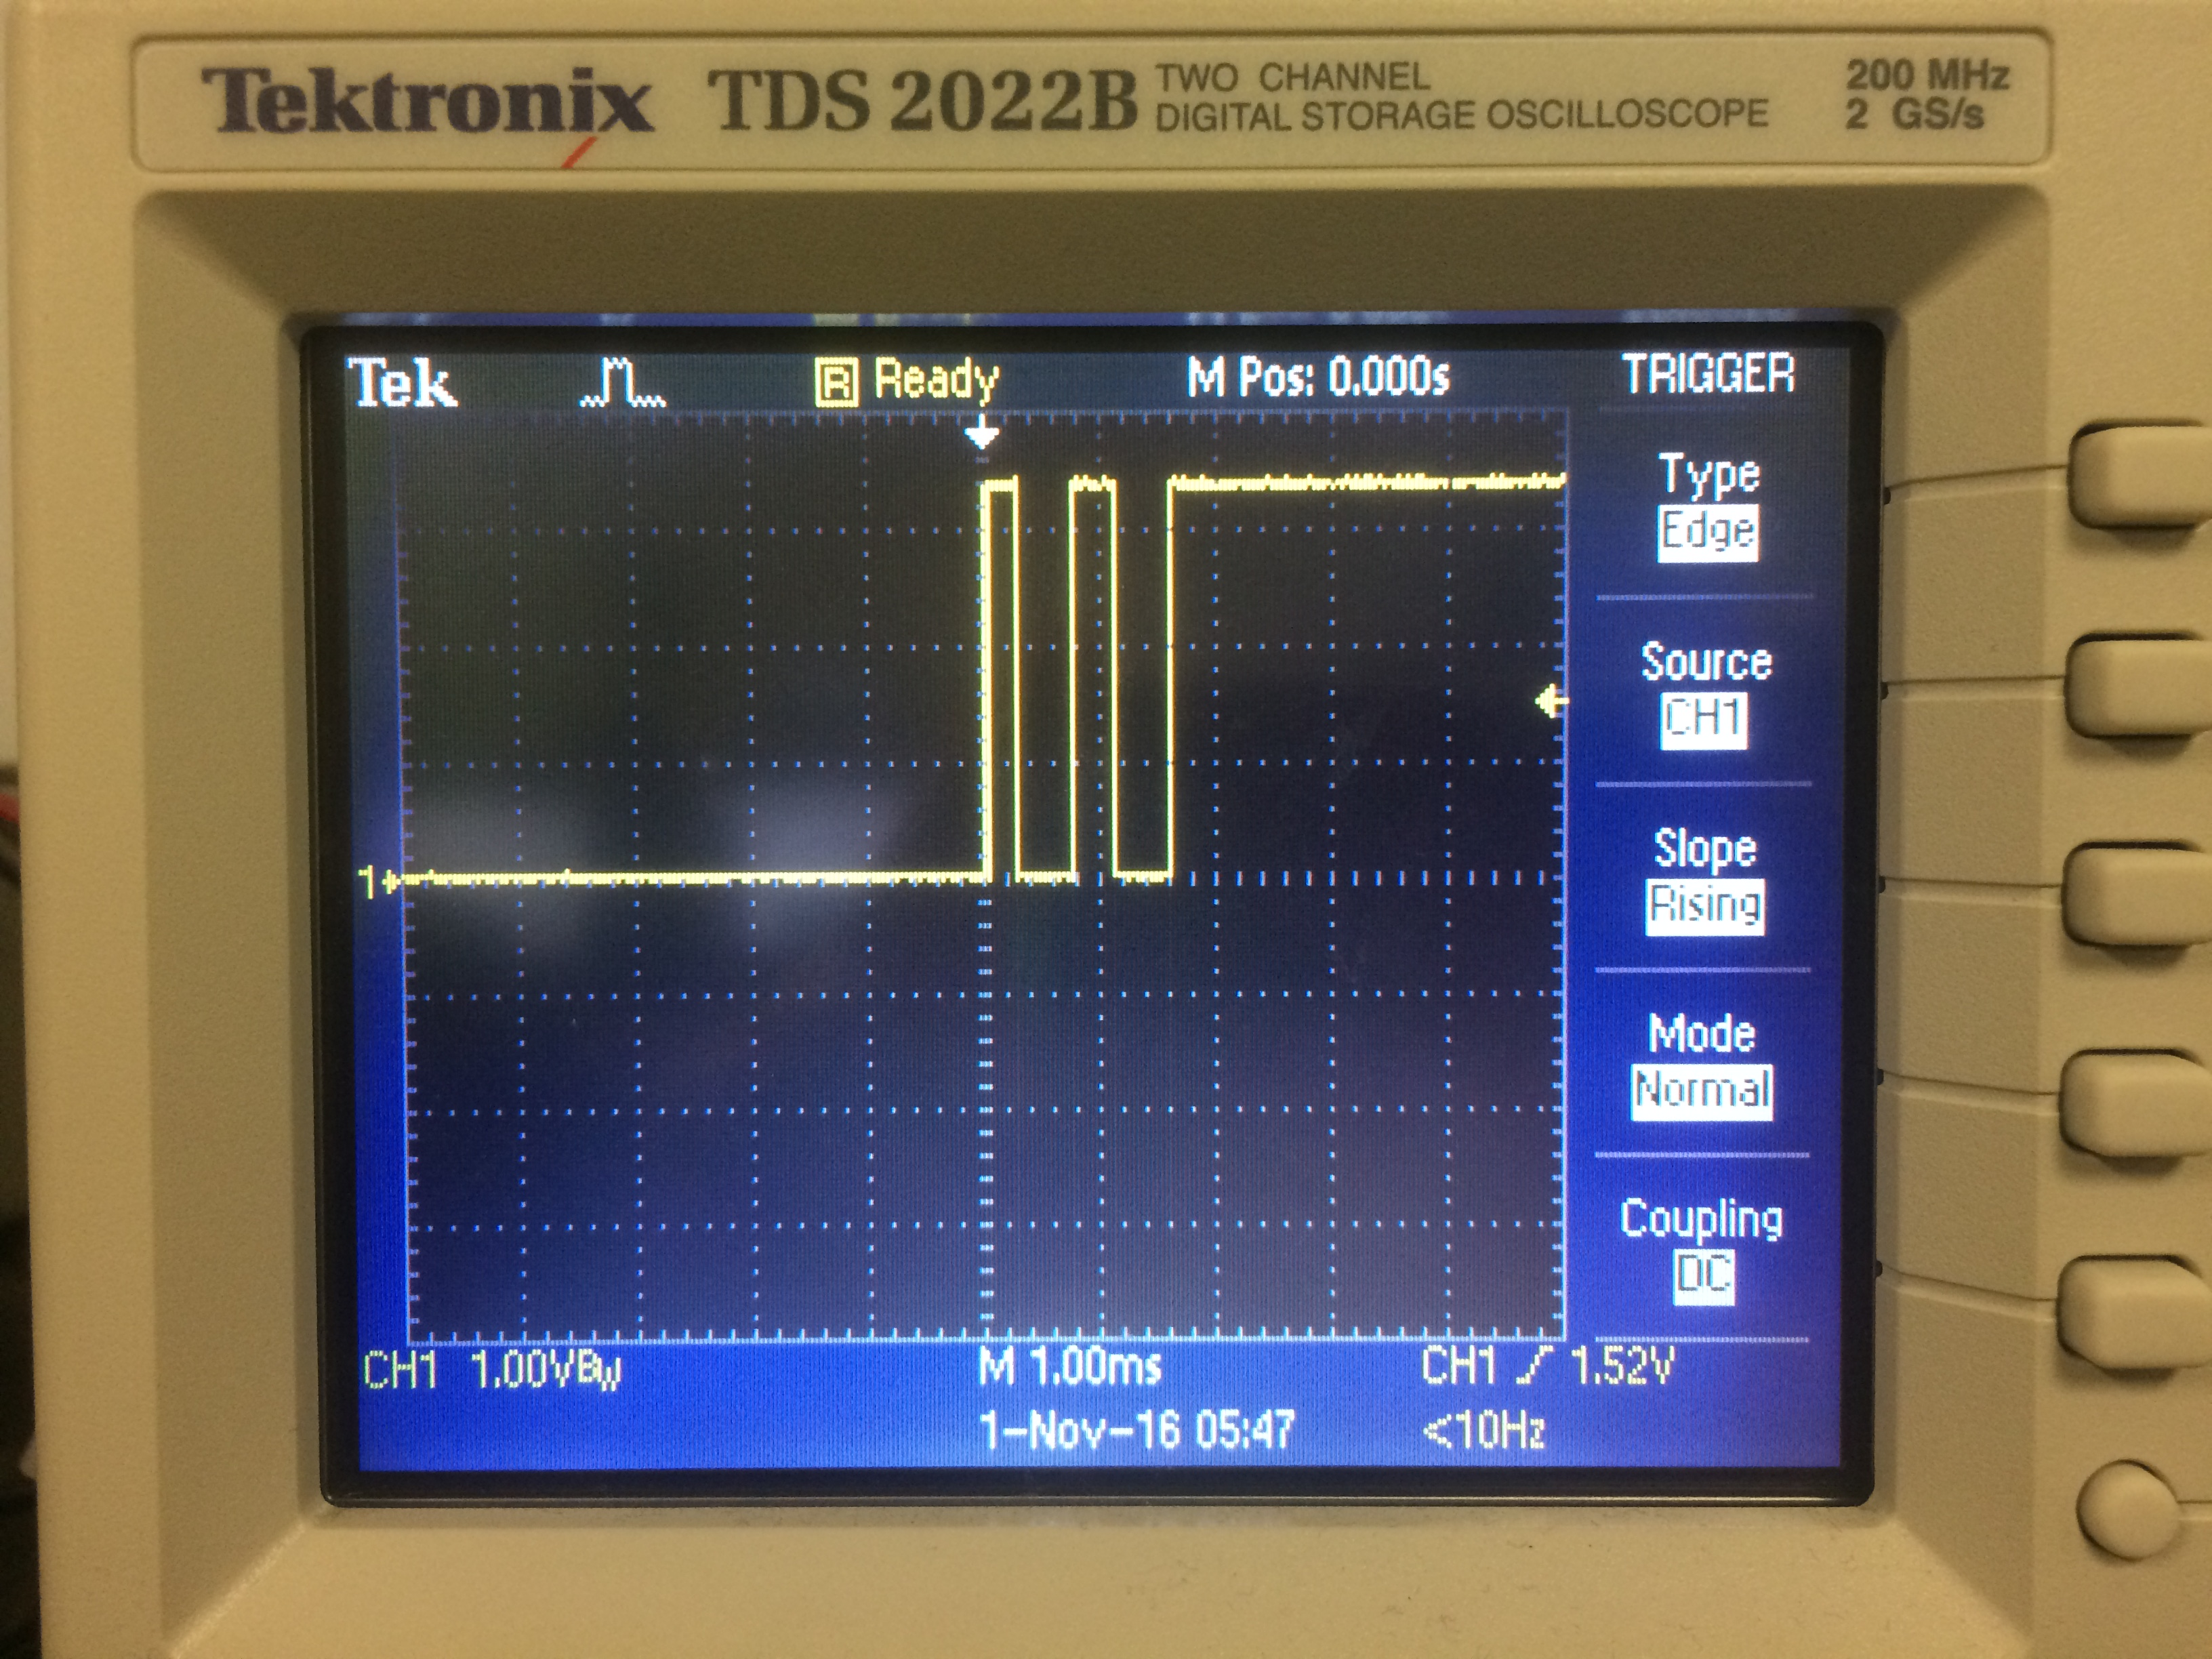
\includegraphics[scale=.1]{IMG_8624.JPG}
      \caption{\textit{Switch Bounce}}
    \end{center}
  \end{figure}

\section*{Conclusion}

  \hspace{15pt}In conclusion, this lab allowed us to expand on our familiarity of sequential circuits
  allowing us to design a half adder, up counter, top level, and a clock divider. We also were able to make a UCF file in order to synthesise Verilog onto the FBGA board for the 
  first time. Finally, the last part of the lab had us analyze the effects of electrical chatter and how adding a synthesizer can reduce the interference.

\section*{Questions}

\begin{enumerate}
  \item \textbf{Include the source code with comments for all modules in lab. You do not have to include test bench
  code. Code without comments will not be accepted!}

  \textit{In the report.}
  
  \item \textbf{Include any UCFs that you wrote or modified.}

  \textit{In the report.}
  
  \item \textbf{Include screenshots of all waveforms captured during simulation in addition to the test bench console
  output for each test bench simulation.}

  \textit{In the report.}
  \textbf{The following are the questions and answers listed in the lab report.}

  \item \textbf{Measure and record the period of each clock signal using the green and yellow markers. 
  Based on you measurements, what frequency do you think the input clock is running at?}
  \vspace{-35pt}
  \begin{center}
    \begin{align*}
      COUNT0 &- 80 ns \\
      COUNT1 &- 160 ns \\
      COUNT2 &- 320 ns \\
      COUNT3 &- 640 ns \\
    \end{align*}
  \end{center}
  \vspace{-35pt}
  ClockIn should be $40 ns$ resulting in a frequency of 25 MHz.
  
  \item \textbf{Open up the test bench file and try to understand what is going on. You should see that the test
  bench produces a Clk signal. What is the frequency of that signal?}
  
  In the test bench, the clock signal is held for 5 ns high and then 5 ns low which would result in a 10 ns cycle. The frequency would then be 100 MHz
  
  \item \textbf{You should also see that the test bench holds the counter in reset for a specific interval of time. How long is that interval?}
  
  The interval is 20 ns
  
  \item \textbf{After reset is de-asserted, the test bench holds the enable LOW for some amount of time before 
  allowing the counter to run. How long is this time period?}
  
  This time period is 20 ns.
  
  \item \textbf{What is this maximum count value and what signal in the waveform could we use to know
  exactly when the counter is going to roll over?}
  
  The maximum count value is f in hexadecimal or 15 in decimal. Whenever Carry3 was HIGH, Count was a max, on the downward edge of Carry3, the Count would reset/roll over
  
  \item \textbf{If we use a 50MHz clock to drive our frequency divider, what rate will the most significant bit
  of the divider oscillate at?}
  
  $f_2 = \dfrac{f_1}{2^n} = \dfrac{50 mHz}{2^{26}} = 0.745 Hz$
  
  %\item \textbf{Make note in you lab write-up how the switches affected the LED outputs.}
  
  The switches slowed down the rate at which the LEDs would count up. The fastest counting up would occur when none of the switches were toggled. The slowest would occur when both switches were toggled. This is due to the how the switches were interpreted into binary. There were two switches $S_0$ and $S_1$ where $S_0$ was of least importance. As the binary value of the switches went up, the speed of the LEDs would slow down.
  
  \item \textbf{Make a note in you lab write up of what what is described in these (Switch Bounce) files.}
  
  It connects J10 to the B4 input on the board. It also connects center to V16 (big center button) on the board.

  \item \textbf{NoDebounce. Does the design work as intended?}
  
  The LEDs are a little glitchy because of multiple rising edges due to electrical chatter. 
  
  \item \textbf{Explain the operation of the circuit described in withDebounce.v}
  
  The input wire goes into two flip flops in order to synchronize the signal and eliminate electrical chatter. Then the signal goes into a binary counter. The LEDs correctly 
  incremented based on the number of times the button was pressed.     
  
\end{enumerate}

\section*{Student Feedback}

\begin{enumerate}
  \item \textbf{What did you like most about the lab assignment and why? What did you like least about it and why?}
  
  In this lab, working with a partner proved to be very beneficial. Our ground circuit on the Logic Analyzer was faulty.

  \item \textbf{Were there any section of the lab manual that were unclear? If so, what was unclear? Do you have any suggestions for improving the clarity?}

  The lab manual was clear in this lab contrary to previous labs.

  \item \textbf{What suggestions do you have to improve the overall lab assignment?}
  
  Better equipment.

\end{enumerate}

\ifx
\begin{thebibliography}{1}
\bibitem{Verilog} Charles Kime \& Thomas Kaminski  \emph{Logic and Computer Design Fundamentals} \\ \hspace{15pt}\textit{http://www.cs.bilkent.edu.tr/~will/courses/CS223/Verilog/LCDF3_Verilog_Ch_4.pdf}
\end{thebibliography}

\section*{Attachments}
%Make sure to change these
Lab Notes, HelloWorld.ic, FooBar.ic
%\fi %comment me out

\begin{thebibliography}{9}
\bibitem{Verilog} Charles Kime & Thomas Kaminski  \emph{Logic and Computer Design Fundamentals} \textit{http://www.cs.bilkent.edu.tr/~will/courses/CS223/Verilog/LCDF3_Verilog_Ch_4.pdf}
\end{thebibliography}

%How to cite
Put your Problem statement here! Example of a Citation\cite[p.219]{Robotics}. Here's Another Citation\cite{Flueck}
\fi
\end{document}
